%
% teil3.tex -- Beispiel-File für Teil 3
%
% (c) 2020 Prof Dr Andreas Müller, Hochschule Rapperswil
%
% !TEX root = ../../buch.tex
% !TEX encoding = UTF-8
%

\section{Komplexe Transformationen auf den Kreis
\label{elektro:section:KreisTrafo}}
\kopfrechts{Kreis Transformationen}

Im Abschnitt \ref{elektro:section:RiemannSatz} wurden die Voraussetzungen für die Anwendung des riemannschen Abbildungssatzes beschrieben.
Dabei wurde erwähnt, dass es keine allgemeine Formel für die Abbildung von beliebigen Gebieten auf den Einheitskreis gibt.
Daher suchen wir nach einer Methode, die uns erlaubt, die Abbildung für beliebige Gebiete zu finden, damit wir die Feldberechnugnen vereinfachen können.

Unser Ziel ist es bekanntlich, Berechnungen anhand des Einheitskreises durchzuführen, da wir dort die Feldgleichungen bereits kennen. 
(Siehe Gleichung \eqref{elektro:equation:potential} und \eqref{elektro:equation:efeld}).
Für eine solche Transformation gibt es mathematisch mehrere Ansätze, die zu einer Lösung führen.
Es wird hier über das Schwarz-Christoffel-Verfahren und über den numerischen Ansatz berichtet, der auf der Finite-Elemente-Methode basiert.
\textcolor{red}{Quelle}

% Hier wird der Ansatz über die Schwarz-Christoffel-Transformationen vorgestellt, die auf einem approximativen Integrationsverfahren basiert.

\subsection{Schwarz-Christoffel-Transformation
\label{elektro:section:SchwarzChristoffel}}
Die Schwarz-Christoffel-Transformation ist ein Verfahren, um den Einheitskreis auf ein Polygon abzubilden. 
Es geht darum, den Rand des Einheitskreises auf den Rand des Polygons abzubilden, sodass die Abbildung konform ist $f: D \rightarrow P $.
Wenn der Einheitskreis $D = {w \in C ; \vert w \vert < 1}$ ist, dann ist der Rand des Einheitskreises $\vert w \vert = 1$, die Bedingung wird nun verwendet um Punkte auf dem Rand des Einheitskreises festzulegen, die auf die Ecken des Polygons abgebildet werden.
Die Punkte auf dem Einheitskreis, die so genannten \emph{Prevertices}, werden als $w_1, w_2, ..., w_n$ bezeichnet, dabei gilt: $\vert w_n \vert = 1$.
Die Prevertices werden als komplexe Zeiger dargestellt, $w_k = e^{\i \theta_k} $.
Die Ecken des Polygons werden als $z_1, z_2, ..., z_n$ bezeichnet.
Und jetzt wird die Funktion $f(w_n) = z_n$ gesucht, welche die $w_n$ auf die $z_n$ abbildet. \textcolor{red}{Laufvariable k oder n ?}
Die Konstruktion beruht auf den bekannten Innenwinkeln der Ecken des Polygons, die als $\alpha_1, \alpha_2, ..., \alpha_n$ bezeichnet werden, und auf den Seitenlängen des Polygons, $L_k = \vert z_{k+1} - z_k \vert$.

Als erster Schritt in der Berechnung wird nun die Ableitung der Schwarz-Christoffel Formel verwendet, da vorerst nur die Richtungsänderung an den Ecken des Polygons von Bedeutung ist. 
\begin{equation}
	f'(w) = C \prod_{k=1}^{n} \biggl(1-\frac{w}{w_k}\biggr)^{\alpha_k-1}
	\label{elektro:equation:SchwarzChristoffelDerivative}
\end{equation}
C ist eine Kostante, die später bestimmt wird und $\alpha_k$ ist bereits bekannt.
Daher fehlen nur noch die Prevertices $w_k$.
Diese werden durch die Seitenlängen des Polygons aufgespürt, da durch die Konformität der Abbildung die Seitenlängen des Polygons erhalten bleiben müssen. 
Damit ohne den Faktor C vorgegangen werden kann, wird das Verhältnis zweier benachbarter Seiten gebildet.
Damit entsteht das folgende Gleichungssystem für die Prevertices $w_k$:
\begin{equation}
	\frac{L_k}{L_1} = \frac{\bigg\vert \int_{w_k}^{w_{k+1}} \prod_{j=1}^{n}(1-\frac{w}{w_j})^{\alpha_j-1} dw \bigg\vert}{\bigg\vert \int_{w_1}^{w_2} \prod_{j=1}^{n}(1-\frac{w}{w_j})^{\alpha_j-1} dw \bigg\vert}
	\label{elektro:equation:SchwarzChristoffelPrevertices}
\end{equation}
Dieses Gleichungssystem ist nichtlinear, weswegen es immer von einem Computer gelöst wird, indem er die Prevertices solange hin und her schiebt bis die Seitenlängenverhältnisse übereinstimmen.

Die gesamte Abbildung wird durch das Integral aller Teile der Ableitung gebildet, wobei die Integrationsgrenze $w_0$ auf einen beliebigen Punkt des Einheitskreises gesetzt werden kann, da die Abbildung bis auf eine Translation eindeutig ist.
\begin{equation}
	f(w) = A + C \int_{w_0}^{w} \prod_{k=1}^{n}(1-\frac{\zeta}{w_k})^{\alpha_k-1} d\zeta
	\label{elektro:equation:SchwarzChristoffel}
\end{equation}

In diesem Anwendungsfall ist vielleicht aufgefallen, dass immer das Feld ausserhalb des Polygons betrachtet wird, daher muss hier noch die feie Unterscheidung gemacht werden, dass die Aussenwinkel betrachtet werden müssen. 
Dazu kommt dass die Fläche des Einheitskreises von innen nach aussen gestülpt werden muss, was wie in Abschnitt \ref{elektro:subsection:Kreisspiegelung} beschrieben durch die Kreisspiegelung erreicht wird. 
\begin{equation}
	f(w) = A + C \int_{w_0}^{w} \frac{1}{{\zeta}^2}\prod_{k=1}^{n}(1-\frac{\zeta}{w_k})^{-\alpha_k-1} d\zeta
	\label{elektro:equation:SchwarzChristoffelExterior}
\end{equation}
Was bedeuten die dazugekommenen Faktoren in der Gleichung \ref{elektro:equation:SchwarzChristoffelExterior}:
\begin{itemize}
	\item $\frac{1}{\zeta^2} $ dieser Faktor sorgt dafür dass der Ursprung des Kreises in die Unendlichkeit gefördert wird.
	\item $-\alpha_k-1$ das Minus vor dem Exponenten sorgt dafür dass die Aussenwinkel des Polygons betrachtet werden.
\end{itemize}

Um das Beschriebene zu veranschaulichen sind in Abbildung \ref{elektro:figure:SchwarzChristoffel_erklaerung} die Prevertices $w_n$, die Ecken des Polygons $z_n$ und die Winkel $\alpha_k$ eingezeichnet.

//TODO: Aussenwinkel korrigieren

\begin{figure}
	\centering
	\includegraphics[width=0.9\textwidth]{papers/elektro/grafik/SC_trafo_erklaerung.png}
	\caption{Prevertices, Ecken und $\alpha_{k}$ abgebildet}
	\label{elektro:figure:SchwarzChristoffel_erklaerung}
\end{figure}



% \subsection{MATLAB Toolbox für Schwarz-Christoffel-Transformationen}
% \label{papers:elektro:subsection:sc-toolbox}


\subsection{Beispiel: Dreiech auf Kreis}
Ein Dreieckige kontour eines ladungsbehafteten Objektes kann als einfaches beispiel vieler Effekte der Transformation zeigen.
Mit der Schwarz-Christoffel Trassformation kann nun der Einheitskreis so transoformiert werden dass desen Rand die Form unseres Dreiecks annimt.
Und damit ein Feld berechnet werden kann das exakt die Form des Dreiecks hat.
Für die Berehcnung der prevertices und alle anderen Paramerter wird das MATLAB Tool benutz das in Abbschnit \ref{papers:elektro:subsection:sc-toolbox} beschirben wurde. \textcolor{red}{ist die beschreibeung des Tools überhaupt nötig ?}
Danach wird die Transformation angewendet und damit kommt das Feld so heraus wie in Abbildung \ref{elektro:figure:SC_triag_trafo} darestellt heraus.

\begin{figure}
	\centering
	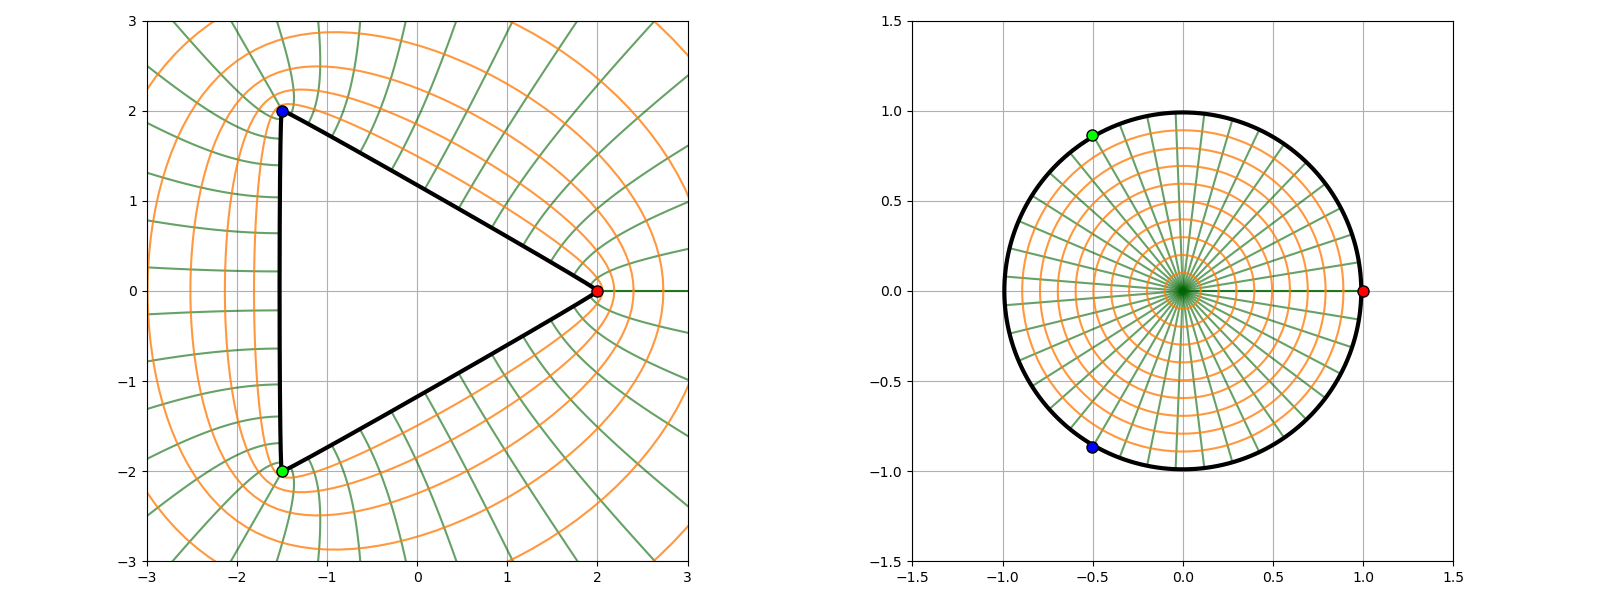
\includegraphics[width=0.9\textwidth]{papers/elektro/grafik/SC_trafo_triag.png}
	\caption{Schwarz-CHristoffel transfomriertes Polygon auf das innere des Einheitskreises}
	\label{elektro:figure:SC_triag_trafo}
\end{figure}

Auf der Abbilung \ref{elektro:figure:SC_triag_trafo} ist zu sehen wie die Feldlinien auf der Oberfläche des Dreiecks senkrecht aufkommen und sich im Raum ausbreiten und dabei auch die Potentiallinen immer senkrecht kreuzen.
Es sind auch die Prevertices auf dem Einheitskreis eingezeichnet die die Punkte markieren die exakt auf die Ecken des Dreiecks transfomiert werden, die farben zeigen welcher punkt auf welche Ecke transformiert wird. 
Dabei fällt auf, dass die Prevertices nicht intuitiv in der selben Richtung wie die Ecken des Dreiecks angeordnet sind, sondern in entgegengesetzten richtungen. 
Die ist auf eine Regel zurpckzuführen die besagt dass die Fläche die bearbeitet wird, im matematischen sinne, immer auf der linken Seite der Kurve liegen muss.
Dies kann so vorgestellt werdem: wenn die laufvariabel des Integrals sich auf der Kurve fortbewegt muss die Fläche die bearbeitet wird immer auf der linken Seite liegen.
Die Verlaufsrichtuung wird also immer so gewählt, dass dies Wahr ist.
Mit einem krleinen Gedanklichen experiment kann nun festgestellt werden dass die Verlaufsrichtung auf dem dreieck im Uhrzeigersinn sein muss und beim Einheitskreis gegen den Uhhrzeigersinn.


Als etwas komplexere Geometrie mit Mehreren Ecken darunter auch welche die einen grösseren Innewinkel als $180^{\circ}$ haben, wird ein Hufeisenförmiges Polygon gezeigt.
\begin{figure}
	\centering
	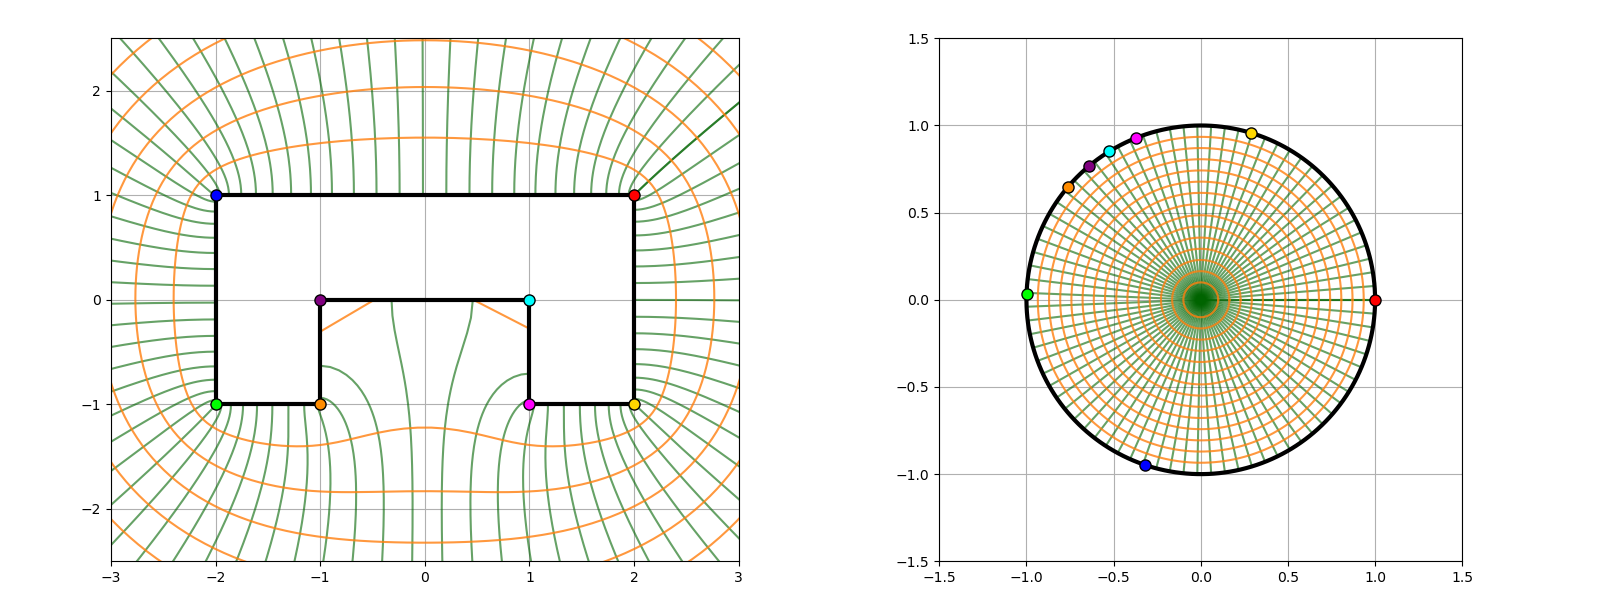
\includegraphics[width=0.9\linewidth]{papers/elektro/grafik/SC_trafo_huf.png}
	\caption{Schwarz-CHristoffel transfomriertes Polygon auf das innere des Einheitskreises}
	\label{elektro:figure:SC_huf_trafo}
\end{figure}

In den Beiden bereits besprochenne Beispielen ist das folgende auch schon zu sehen aber hier kommt noch ein etwas anschaulicheres Beispie, in Abbildung \ref{elektro:figure:SC_star_trafo} sind drei verschiedene Winkel zu finden, die alle eine andere konzentration an Feldlinen aufweisen die senkrecht dort wufkomen.
Bei spitzen winkkeln ist zu sehen das die Feldlinen näher beieinander sind und bei den stumpferen oder sogar überstumpfen Winkeln ist zu sehen dass die Feldlinen weiter auseinander liegen.
Dies ist auf die Ladungsverteilung zurückzuführen die sich auf dem Objekt verteilt.
Bei spitzeren winkeln hat es weniger platz zwischen den ebieden Kanten und LAdungsträger drücken die vor ihnen liegenden Ladungsträger näher zusammen, was zu einer höheren Ladungsdichte an den spitzen führt.
Bei den stumpferen Winkeln ist es genau umgekehrt, dort hat es mehr Platz und die Ladungsträger können sich weiter auseinander verteilen, da dies sowieso das ist was ladungsträger mit gleicher polarität am liebsten tun. 
Genau wie die E-Feldlinen die sich gegenseitig abstossen und sich so weit wie möglich voneinander entfernen.

\begin{figure}
	\centering
	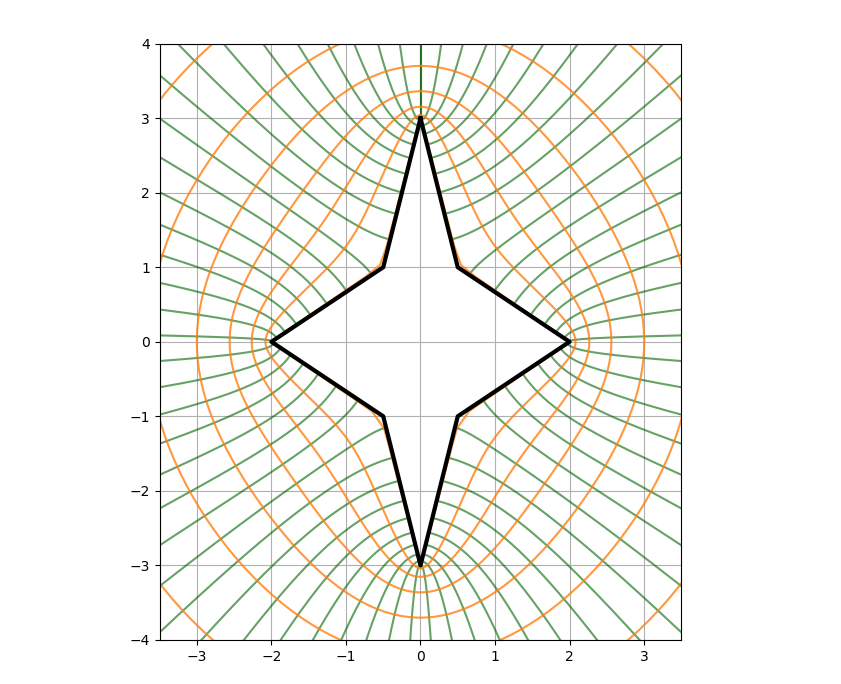
\includegraphics[width=0.9\linewidth]{papers/elektro/grafik/SC_trafo_star.png}
	\caption{Sternförmige Kontour mit verschiedenen Innenwinkeln}
	\label{elektro:figure:SC_star_trafo}
\end{figure}

Diese Spitzeneffekte sind nicht auf die Elektrostatik beschränkt sondern kommen in allen Bereichen der Physik vor.
In der Mechanik ist es das gleiche Prinzip, dass sich Kräfte an den Spitzen von Objekten konzentrieren und dort zu einer höheren Belastung führen.
In Abbildung \ref{elektro:figure:mech_triag} ist ein Beispiel zu sehen wie sich die Kräfte an den Spitzen eines Dreiecks konzentrieren.

\begin{figure}
	\centering
	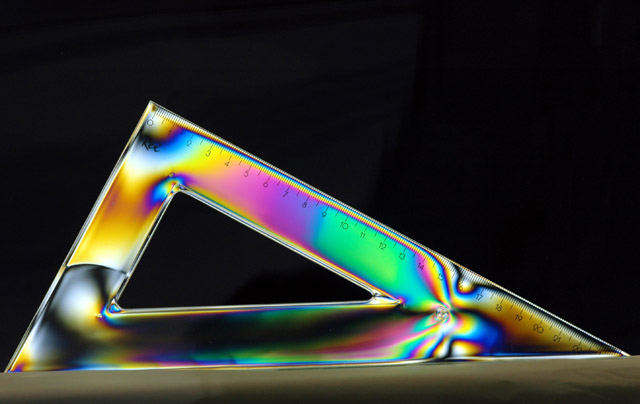
\includegraphics[width=0.9\linewidth]{papers/elektro/grafik/mech_triag.png}
	\caption{Kraftkonzentration an den Spitzen eines Dreiecks}
	\cite[Bild Quelle]{elektro:mech_triag}
	\label{elektro:figure:mech_triag}
\end{figure}
